\documentclass[letterpaper, 12pt]{article}
\usepackage[american]{babel}
\usepackage[utf8]{inputenc}
\usepackage[citestyle=apa,style=apa,backend=biber]{biblatex}
\usepackage[margin=1in]{geometry}
\usepackage{graphicx}
\usepackage{caption}
\usepackage{float}
\setlength\bibitemsep{2\itemsep}
\DeclareLanguageMapping{american}{american-apa}
\addbibresource{bibliography.bib}

\begin{document}
\begin{titlepage}
\centering
	\vspace*{5.75cm}
	{\huge\bfseries Project proposal\par}
	\vspace{2cm}
	Blair Urish\\
	Dan Wagner\\
	Kansas State University\\
	College of Engineering\\
	Department of Computer Science\\
	\vspace{1cm}
	Dr. Bin Liu\\
	Professor\\
	Department of Chemical Engineering\\
	\vspace{1cm}
	October 29, 2017
\end{titlepage}

\begin{abstract}
\thispagestyle{plain}
\begin{flushleft}
	Abstract goes here if we need it.
\end{flushleft}
\end{abstract}
~\newpage

\begin{flushleft}

\section*{Introduction}

\subsection*{Background Research}
Many fields require materials with properties that often conflict or trade off with one another.  Examples of such properties are low density, high strength, and high flexibility.  In most cases, it is difficult or impossible for traditional materials to exhibit combinations of these properties.

\section*{Methodology}
 A global single-population master-slave genetic algorithm was chosen as the best method of parallelization. The master node receives a population and divides individuals between the slave nodes.  Slave nodes will evaluate the fitness of individuals they receive and send the results back to the master node.  A visualization of this technique can be seen below.
 
 \begin{figure}[H]
 	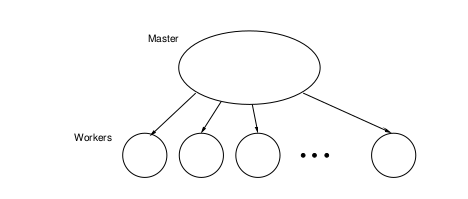
\includegraphics[width=\linewidth,height=10cm,keepaspectratio]{model.png}
 	\caption[Master-Slave Genetic Algorithm Implementation]{Master-Slave Distributed Genetic Algorithm. Adapted from \cite{cantu1998survey}}
 	\label{fig:arch}
 \end{figure}

~\newline We will realize this solution using several nodes on the Beocat supercomputing cluster.   One computing node will be designated as the master node, while several other nodes will be the slave nodes.  The master node will receive the population of randomly generated parameter sets and the training set provided.  It will partition the population into subsets to send to the slave nodes for evaluation.  Each slave node will evaluate the fitness of each individual within their subset and transfer the results to the master node for modification via trait crossover and mutation. The best one hundred individuals are retained for subsequent generations.\\

~\newline ~\newline ~\newline 
This process will continue until the genetic algorithm fails to return better individuals than the previous run.  At this convergence step, the twenty best individuals are selected to be locally minimized by using the Simplex method.  Finally, the most optimized individual results in the best set of parameters for this generation.

\begin{figure}[H]
	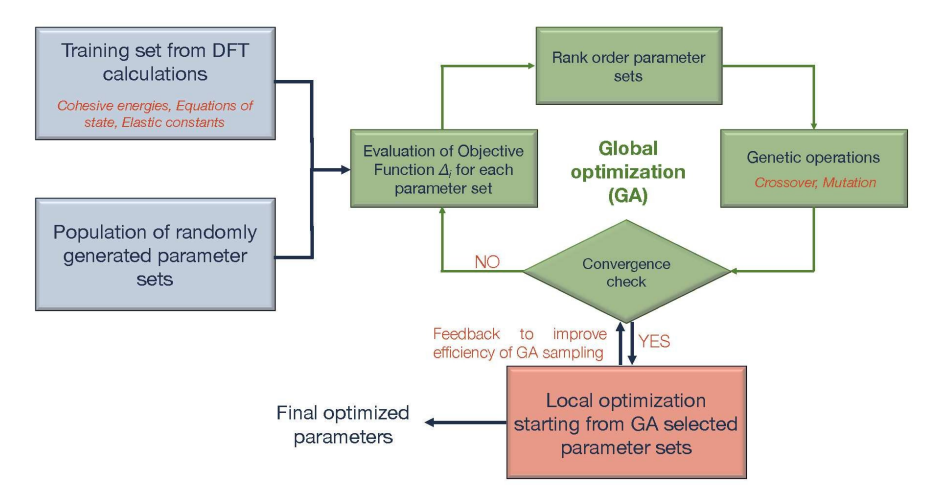
\includegraphics[width=\linewidth,height=10cm,keepaspectratio]{flowchart.png}
	\caption[Overall Flow of Genetic Algorithm Process]{Overall Flow of Genetic Algorithm Process. Adapted from \cite{C7NR06038F}}
	\label{fig:arch}
\end{figure}


\section*{Conclusion}

\newpage
\printbibliography

\end{flushleft}
\end{document}
